\documentclass{article}
\usepackage[T1]{fontenc}
\usepackage{lmodern}
\usepackage{graphicx}
\usepackage{amsmath,amssymb}
\usepackage[a4paper,margin=2cm]{geometry}
\usepackage[absolute,overlay]{textpos}
\setlength{\TPHorizModule}{1mm}
\setlength{\TPVertModule}{1mm}
\usepackage[indonesian]{babel}
\usepackage{hyperref}
\setlength{\emergencystretch}{2em}
% unit: Halaman 8

\begin{document}

% === Halaman 8 (python/native) ===

8

2.

Known-plaintext attack 


Diberikan sejumlah pasangan plainteks dan cipherteks yang 

berkoresponden:    


   P1  dan C1 = Ek(P1),  P2 dan C2 = Ek(P2),  … ,  …, Pi dan Ci = Ek(Pi) 


Deduksi:  k untuk mendapatkan Pi+1 dari Ci+1 = Ek(Pi+1).

Sumber: https://www.hackers-arise.com/post/2019/04/30/cryptography-basics-part-

2-attack-models-for-cryptanalysis

% deskripsi: gambar native xref 105
\noindent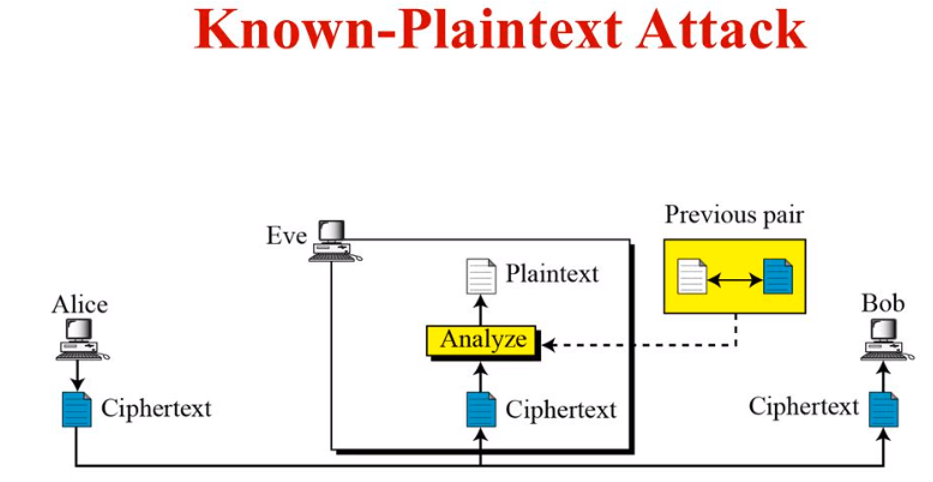
\includegraphics[width=0.85\textwidth]{../../images/python/page_008_img_01.png}

\end{document}
